\documentclass[tikz,convert={density=600,size=1080x800,outext=.png}]{standalone}
\usepackage{tikz}
\usepackage{ifthen}
\usepackage{etoolbox}
\usetikzlibrary{matrix,arrows.meta,bending,positioning,calc}

% !TEX root = relative/or/absolute/path/to/root/file.tex


\tikzset{
    table relation/.style={
        %below=of game,
        nodes={draw=black, text width=5cm}, % Change the text width here to reduce the width of all tables
        row 1/.style={nodes={align=center, fill=lightgray, font=\bfseries}},
        row/.style={anchor=base east}
    },
    booking table/.style={
        nodes={draw=black, text width=6cm}, % Change the text width here to increase the width of the Flight table
        row 1/.style={nodes={align=center, fill=lightgray, font=\bfseries}},
        row/.style={anchor=base east}
    },
    flight table/.style={
        nodes={draw=black, text width=8cm}, % Change the text width here to increase the width of the Flight table
        row 1/.style={nodes={align=center, fill=lightgray, font=\bfseries}},
        row/.style={anchor=base east}
    },
    -|-/.style={
        to path={
            (\tikztostart) -| ($(\tikztostart)!#1!(\tikztotarget)$) |- (\tikztotarget)
            \tikztonodes
        }
    },
    -|-/.default=0.5,
}
\begin{document}


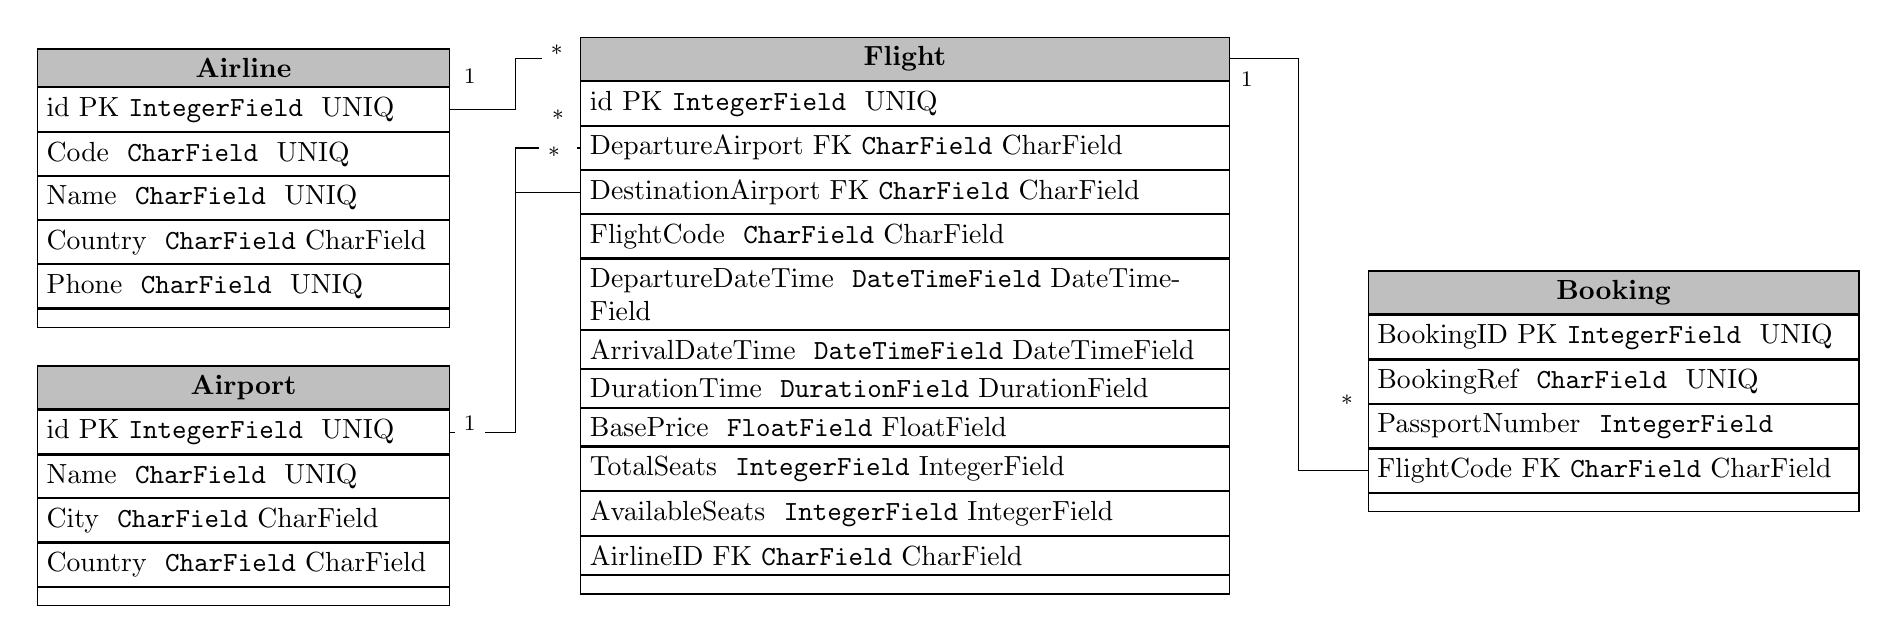
\begin{tikzpicture}[scale=1.2]
    % DRAW TABLES
    
    % Please note, in general you'll see the commands:
    % \node (tx) {Table Name};\\
    % as well as
    % \xappto\matrixcontent{\expandonce{\node} (t0_\x) {\x\ \y\ \expandonce{\texttt}{\z}};\\}

    % tx is essentially the identifier for this table and is used
    % when it comes to drawing connections between the tables
    % individual rows are denoted as t0_attributeName
    % make sure you update both commands when you choose an id for your table
    
    % Example:
    % First table has identifier t1 and one attribute name is
    % cost
    % the id for that row is t1_cost


    % TABLE 1
    % Set up matrix content
    \let\matrixcontent\empty

    % ~~~ ATTRIBUTES OF THE TABLE GO HERE ~~~
    % <attribute name>/<PK or FK label (optional)>/<data type>
    \foreach \x/\y/\z/\u in {
        id/PK/IntegerField/ UNIQ,
        Code//CharField/ UNIQ,
        Name//CharField/ UNIQ,
        Country//CharField,
        Phone//CharField/ UNIQ,
    } {
        \xappto\matrixcontent{\expandonce{\node} (t1_\x) {\x\ \y\ \expandonce{\texttt}{\z} \u};\\}
    }
    \matrix[
        matrix of nodes,
        table relation,
    ] at (0, 1.15) { % Position of the table is (0, 0)
        \node (t1) {Airline};\\
        \matrixcontent
    };\\

    
    % TABLE 2
    % Set up matrix content
    \let\matrixcontent\empty

    % ~~~ ATTRIBUTES OF THE TABLE GO HERE ~~~
    % <attribute name>/<PK or FK label (optional)>/<data type>
    \foreach \x/\y/\z/\u in {
        id/PK/IntegerField/ UNIQ,
        DepartureAirport/FK/CharField,
        DestinationAirport/FK/CharField,
        FlightCode//CharField,
        DepartureDateTime//DateTimeField,
        ArrivalDateTime//DateTimeField,
        DurationTime//DurationField,
        BasePrice//FloatField,
        TotalSeats//IntegerField,
        AvailableSeats//IntegerField,
        AirlineID/FK/CharField,
    } {
        \xappto\matrixcontent{\expandonce{\node} (t2_\x) {\x\ \y\ \expandonce{\texttt}{\z} \u};\\}
    }
    \matrix[
        matrix of nodes,
        flight table,
    ] at (7, -0.2) {
        \node (t2) {Flight};\\
        \matrixcontent
    };\\

   

    \let\matrixcontent\empty

    \foreach \x/\y/\z/\u in {
        id/PK/IntegerField/ UNIQ,
        Name//CharField/ UNIQ,
        City//CharField,
        Country//CharField,
    } {
        \xappto\matrixcontent{\expandonce{\node} (t3_\x) {\x\ \y\ \expandonce{\texttt}{\z} \u};\\}
    }
    \matrix[
        matrix of nodes,
        table relation,
    ] at (0, -2) { % Position of the table is (0, 0)
        \node (t3) {Airport};\\
        \matrixcontent
    };\\

    \let\matrixcontent\empty

    \foreach \x/\y/\z/\u in {
       BookingID/PK/IntegerField/ UNIQ,
       BookingRef//CharField/ UNIQ,
        PassportNumber//IntegerField/ ,
        FlightCode/FK/CharField,
    } {
        \xappto\matrixcontent{\expandonce{\node} (t4_\x) {\x\ \y\ \expandonce{\texttt}{\z} \u};\\}
    }
    \matrix[
        matrix of nodes,
        booking table,
    ] at (14.5, -1) { % Position of the table is (0, 0)
        \node (t4) {Booking};\\
        \matrixcontent
    };\\


    % DRAW RELATIONS BETWEEN THEM
    % This is finicky, but please bear with
    % \x - the attribute which acts as a foreign key to another table
    % \y - the table represented by the above FK

    % \p - Positioning for line endpt at \x (which side of the box to draw the line on).
    % \q - As above, for \y

    % \a - \x endpoint label (to denote quantity in the relation)
    % \b - \y endpoint label (to denote quantity in the relation)

    % note: \p and \q should be denoted as a compass value, e.g., north for top, south for bottom, west for left, east for right
    % bottom.
   \foreach \x/\p/\a/\y/\q/\b in {
        t1_id/east/1/t2/west/*
    } {
        \draw[] (\x.\p) to[-|-] (\y.\q);
        \node[fill=white,align=center, yshift=9.25pt] at ($(\x.\p)!0.15!(\y.\q)$) {\footnotesize\a};
        \node[fill=white,align=center, yshift=4.75pt] at ($(\x.\p)!0.85!(\y.\q)$) {\footnotesize\b};
    }
    \foreach \x/\p/\a/\y/\q/\b in {
       t3_id/east/1/t2_DepartureAirport/west/*,
       t3_id/east/1/t2_DestinationAirport/west/*
    } {
        \draw[] (\x.\p) to[-|-] (\y.\q);
        \node[fill=white,align=center, yshift=-10pt] at ($(\x.\p)!0.15!(\y.\q)$) {\footnotesize\a};
        \node[fill=white,align=center, yshift=26.25pt, xshift=-1pt] at ($(\x.\p)!0.85!(\y.\q)$) {\footnotesize\b};
    }
    \foreach \x/\p/\a/\y/\q/\b in {
        t4_FlightCode/west/*/t2/east/1
    } {
        \draw[] (\x.\p) to[-|-] (\y.\q);
        \node[fill=white,align=center, yshift=2pt] at ($(\x.\p)!0.15!(\y.\q)$) {\footnotesize\a};
        \node[fill=white,align=center, yshift=15pt] at ($(\x.\p)!0.85!(\y.\q)$) {\footnotesize\b};
    }

\end{tikzpicture}
\end{document}